\documentclass[11pt]{article}

\usepackage[utf8]{inputenc}
\usepackage[english]{babel}

\usepackage{mathtools}

\usepackage{setspace}
\onehalfspacing
\usepackage{subcaption}

\usepackage{amsfonts}
\usepackage{amsmath}
\usepackage{amsthm}
\usepackage{indentfirst}
\newtheorem{theorem}{Theorem}
\newtheorem{lemma}{Lemma}
\newtheorem{example}{Example}
\newtheorem{definition}{Definition}
\newtheorem{remark}{Remark}
\newtheorem{corollary}{Corollary}

\newtheorem*{theorem*}{Theorem}
\newtheorem*{lemma*}{Lemma}
\newtheorem*{example*}{Example}
\newtheorem*{definition*}{Definition}
\newtheorem*{remark*}{Remark}
\newtheorem*{corollary*}{Corollary}

%\usepackage{booktabs, caption, graphicx, float}
%\usepackage{subcaption}
%\captionsetup{tableposition=top,figureposition=bottom,font=small}

\usepackage{comment}
\usepackage{multirow}
\usepackage{array}

\newcolumntype{C}[1]{>{\centering\let\newline\\\arraybackslash\hspace{0pt}}m{#1}}
\DeclarePairedDelimiter\floor{\lfloor}{\rfloor}

\usepackage[hidelinks]{hyperref}

\usepackage{geometry}
\geometry{a4paper, top=3cm,bottom=3cm,left=3cm,right=3cm,%
			heightrounded}
\usepackage{upgreek}
\usepackage{xparse}
\usepackage{listings}
\NewDocumentCommand{\codeword}{v}{%
	\texttt{\textcolor{black}{#1}}%
}

\newcommand{\prepos}[3]{${}_{\mathbf{#2}}{\mathbf{#1}}_{#3}$}
\newcommand{\preposm}[3]{{}_{\mathbf{#2}}{\mathbf{#1}}_{#3}}



\newcommand{\Rnum}{\mathbb{R}} % Symbol fo the real numbers set
\newcommand{\mat}[1]{\ensuremath{\begin{bmatrix}#1\end{bmatrix}}}	% matrix
\newcommand{\myparagraph}[1]{\paragraph{#1}\mbox{}\\}

%Dummy text
\usepackage{lipsum}

%Changing headers and footers
\usepackage{fancyhdr}
\pagestyle{fancy}
\fancyhf{}
\rhead{\textit{\thepage}}
\lhead{\textit{Kinematics and Dynamics Lab}}

%For inserting the code
\usepackage{fancyvrb}

%For bold math symbols
\usepackage{bm}

%For multicolumns
\usepackage{multicol}

% Norm and abs delimiter
\usepackage{mathtools}
\DeclarePairedDelimiter{\abs}{\lvert}{\rvert}
\DeclarePairedDelimiterX{\norm}[1]{\lVert}{\rVert}{#1}

\setcounter{section}{-1}

% Argmin/Argmax
\DeclareMathOperator*{\argmax}{argmax}
\DeclareMathOperator*{\argmin}{argmin}

% Enumerate
\usepackage{enumitem}

% Code
\usepackage{algorithm}
\usepackage[noend]{algpseudocode}
\usepackage{etoolbox}

% Longtable
\usepackage{longtable}
\usepackage{fancyvrb}
% SI units
\usepackage{siunitx}
\sisetup{output-exponent-marker=\ensuremath{\mathrm{e}}}

% Colours in equations
\usepackage{xcolor}

\title{LAB 1: Kinematics and Dynamics Lab: Simulation of a 4-DoF Serial Manipulator}
\author{Michele Focchi and Octavio Villarreal}
\date{}

\begin{document}
\maketitle
\noindent
The goals of this assignment are:
\begin{itemize}
    \item learning the basic procedure to visualize a robot model using the Unified Robot Description Format (URDF)
    \item compute and visualize the direct/inverse kinematics of a 4-DoF serial manipulator 
    \item compute and analyze the forward/inverse dynamics of a 4-DoF serial manipulator using the Recursive Newton-Euler Algorithm (RNEA)
\end{itemize}

\noindent
Tools that we are going to be using in this lab (all open-source):
\begin{itemize}
	\item Python programming (2.7, 3.5)\footnote{https://docs.python.org/2.7/}
	\item Robot Operating System (ROS)\footnote{https://www.ros.org/}
	\item Pinocchio Library for Rigid Body Dynamics Algorithms\footnote{https://github.com/stack-of-tasks/pinocchio}
	\item Locosim\footnote{https://github.com/mfocchi/locosim}
\end{itemize}
%
%
%\noindent
The goal of this assignment is to arrive to simulate the behavior of a 4-DoF anthropomorphic robot manipulator under zero-torque at the joints (i.e., free-falling under the effect of gravity which is the only force making work on the robot). Initially we will learn how to describe a robot using the URDF convention, such that ROS is able to "understand" and visualize our robot using the visualizer tool in RVIZ.\footnote{https://dl.acm.org/doi/abs/10.1007/s11235-015-0034-5} Secondly, we will proceed to develop code in Python to compute the direct and inverse kinematics functions of  our robot manipulator and we will design a simple trajectory for our robot to follow based on polynomials. Finally, we will write functions to compute both the forward (to simulate) and the inverse dynamics (to control) of our robot manipulator using the RNEA.  Based on RNEA, we will compute separately each of the terms of the dynamics equation ($\mathbf{M}$, $\mathbf{h}$ and $\mathbf{g}$) and perform analysis on them. For both the kinematics and dynamics parts, we will compare our results with the built-in functions of the Pinocchio library to verify the correctness of our computations.

%
\section{Preliminaries}
We are going to be using functions and interfaces written in the locosim package installed in the provided virtual machine (VM) for the course. Locosim is stored as a github\footnote{https://git-scm.com/} repository, and we have created a branch containing the files needed for this lab, but we need to get them in our VM to do so, follow these steps:

\begin{enumerate}
	\item Open a new terminal inside of the VM (either by clicking on the icon of the launcher on the left or by hitting the keyboard shortcut \codeword{Ctrl + Alt + T})
	\item If you need to update the software in the terminal type the following commands
	
	\begin{verbatim}
		cd ros_ws/src/locosim/
		git fetch 
		git checkout develop
		git submodule update --init --recursive
		cd ~/ros_ws
		catkin_make install
	\end{verbatim}

\end{enumerate}

As you see, the last command is a compilation command. Indeed, despite all the labs are written in Python and located in the \codeword{robot_control} folder, there is a low level controller called \codeword{ros_impedance_controller} that receives joint commands from Python and sent them to Gazebo (in the labs where a Gazebo simulator is used). This node is written in C++ and needs to be compiled (and installed in the folder where ROS looks to find the nodes that is stored in the environment variable  \codeword{ROS_PACKAGE_PATH}). 
%
\section{Robot URDF description file and visualization}
%
In this part of the lab we are going to visualize our 4-DoF manipulator using the previously mentioned software tools.

\textbf{1.1 Basic geometry description.} Go to the folder that contains the files corresponding the robot description by typing the following commands on the terminal:


\begin{verbatim}
	cd ~/ros_ws/src/locosim/robot_urdf
\end{verbatim}

 If you do not find \codeword{~} replace it with \codeword{/home/student}.
Let's start by inspecting a file that describe a robot made of regular geometries (a box and a cylinder). Type on the terminal:

\begin{verbatim}
	gedit simple_geometry.urdf
\end{verbatim}

As mentioned, a robot is described in robot using a URDF file, which is scripted using the metalanguage \codeword{xml}, and specific \codeword{xml} macros (i.e., \codeword{xacro}). We can both use the extension \codeword{*.urdf} or \codeword{*.xacro}, however, when dealing with large models a combination of both might be required since \codeword{xacro} files allowed for modularity, but some CAD software outputs directly a \codeword{urdf} file. In general, you use \codeword{xacro}  to assemble  parametrized \codeword{urdf}  of the subparts of a robot. For instance in the case of a legged robot, you can define the  \codeword{urdf} for a generic leg and parametrize it with its location along the trunk, without copying and pasting code. However, in this class, we will not use this feature and you will find only \codeword{urdf} files in the folder. 
Inspect the \textit{simple\_geometry} file and try to understand what each line describes. How are the links described? Which parameters need to be described per link? How are joints defined? \footnote{For an in-depth explanation on how ROS works and check this useful book: Mastering ROS for Robotics	Programming, Lentin Joseph, pag. 61.}. 

The link tag represents a single link of a robot. Using this tag, we
can model a robot link and its dynamic properties. The syntax is as follows:
	
\begin{Verbatim}	
<link name="name of the link">
	<inertial>...........</inertial>
	<visual> ............</visual>
	<collision>..........</collision>
</link>
\end{Verbatim}

The \textit{Visual} section represents the real link of the robot, and the area surrounding the real link
is the \textit{Collision} section. The Collision section encapsulates the real link to
detect collision before hitting the real link. The inertial tag defines the mass, the location of the center of mass and the inertia tensor of the link (about the CoM). These parameters are usually obtained by CAD.

\begin{figure}[H]
	\centering
	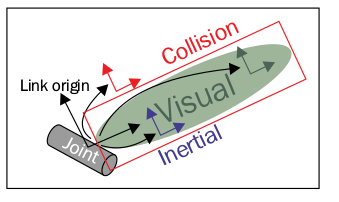
\includegraphics[width=6cm]{pics/link.png}
	\caption{Visualization of a URDF link}
	\label{fig:link}
\end{figure}

The joint tag represents a robot joint. e should specify the type of joint (revolute, prismatic, floating, fixed, continuous).  
A  joint is formed between two links; the first is called the Parent link
and the second is the Child link. The syntax is as follows:

\begin{Verbatim}	
<joint name="name of the joint" type="type of the joint">
	<parent link="link1"/>
	<child link="link2"/>
	<origin  xyz="..." rpy="..."/>
	<axis xyz="0 0 1"/>
	<limit effort .... />
</joint>
\end{Verbatim}

We can specify the kinematics of the robot setting the location of the joint frame with respect to the supporting link with the tag \codeword{origin} that represents the \textit{rigid transform} with respect to the supporting link frame. To summarize: from a link frame $i$ with a rigid transform we find the frame of the next joint ($i+1$). Then if the joint variable  is \textit{zero}, the joint $i+1$ frame is coincident with the link frame $i+1$ that the joint is moving. If the joint moves  then the link $i+1$ frame and the joint $i+1$ frame no longer coincide and are linked by an additional transformation (e.g. a pure elementary rotation about the joint axis in the  case of a revolute joint \footnote{In the case of a revolute joint the origin of the joint and link frame always coincide.}) due to the joint motion. Note that the joint axis is defined with respect to the parent link (e.g. $i$) not with respect to the world frame!
We can also set the limits of the joint movement and
its velocity and the effort (i.e. force or torque).
 The following is an illustration of a joint and
its link:

\begin{figure}[H]
	\centering
	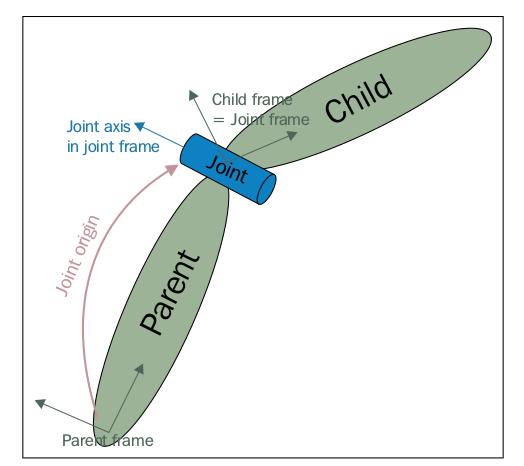
\includegraphics[width=6cm]{pics/joint.png}
	\caption{Visualization of a URDF joint.}
	\label{fig:link}
\end{figure}

In this picture the frame supporting the \textit{child} link is coincident with the joint frame so it means that the joint variable is 0.
The position / orientation of the joint frame is expressed via a rigid transform (with the tag origin) with  respect to the \textit{parent} link frame. 
%The axis of the joint is also defined with respect to the parent link frame (not the %inertial frame!). 
\\



\textbf{1.2 Use an stl mesh file to describe a link.} We can use .stl files to specify the geometry of the link instead of using basic geometries such as a cilinder or a block. The .stl format is a common extension used in CAD softwares such as SolidWorks to store rigid parts of a mechanical design. However, when using stl files, one needs to be careful to not use an excessive number of polygons to describe the part \footnote{People use Meshlab to reduce mesh complexity from a detailed CAD}, since this might cause the simulation to slow down significantly. The file \codeword{ur4_2links.urdf} contains to links associated to a mesh stl file. Inspect the \codeword{ur4_2links.urdf} by typing in the terminal (you can either open a new terminal or kill the process in the previous one by hitting \codeword{Ctrl + C})
%
\begin{verbatim}
	gedit ur4_2links.urdf
\end{verbatim}
%
You will notice that the file contains more details and parameters per link and joint. What can they represent? Where are these values obtained from? Are they referred to a specific reference frame? Inspect each line of the file and try to understand the function of each 
of the tags. Check how the rigid (homogeneous) transform is set for the \textit{shoulder\_pan\_joint}  with respect to the supporting \textit{base\_link}. Check also how the dynamic parameters (mass, Center of Mass and inertia tensor) are defined for the link, with respect to the link frame.\\




\textbf{1.3 Visualizing a model described by a URDF in RVIZ.} The basic unit of development in ROS is the node. A node is nothing else than a process that performs computations. It can be created in multiple languages and interfaces such as Python and C++. Nodes communicate through messages by either using a publisher-subscriber (synchronous)\footnote{http://wiki.ros.org/ROS/Tutorials/WritingPublisherSubscriber(python)} or a request-reply (asynchronous)\footnote{http://wiki.ros.org/ROS/Tutorials/WritingServiceClient(python)} scheme. In this lab session we will use the former one, and locosim already provides a dedicated function to publish the state of the joints during runtime and make them available to the visualizer node running RVIZ. One can run each node separately using the terminal command \codeword{rosrun}\footnote{http://wiki.ros.org/rosbash\#rosrun}, however, a more convenient way is to setup a launch file and run multiple nodes with only with terminal command (namely, \codeword{roslaunch}\footnote{http://wiki.ros.org/roslaunch}). Let us inspect the launch file to visualize our examples of URDF files. In a terminal type:
%
\begin{verbatim}
	cd ~/ros_ws/src/locosim/ros_impedance_controller/launch
	gedit visualize.launch
\end{verbatim}
%
Once the file has been inspected,  run the following command in the terminal to load the URDF of the \codeword{simple_geometry} robot:

\footnotesize
\begin{verbatim}
	roslaunch ros_impedance_controller visualize.launch robot_name:=simple_geometry 
\end{verbatim}
\normalsize

 You can play around with the value of the only joint (shoulder\_pan\_joint) present in the model, using the slider input in the GUI. It is possible to visualize the link frames, adding the TF plugin in RVIZ. Stop the process by hitting \codeword{Ctrl + C} in the terminal in which you ran the previous launch file. 
Now let's visualize a one-joint two-link manipulator by typing the following command:
%
%
\footnotesize
\begin{verbatim}
	roslaunch ros_impedance_controller visualize.launch robot_name:=ur4_2links  
\end{verbatim} 
\normalsize
Again, you will visualize the described model and you can modify the value of the only joint to make the shoulder link move. Note that until now we were only \textit{visualizing} a predefined joint motion, note that we would need to add a \textit{trasmission} to the joint if we want to be able to control it in a simulator (i.e. sending torques to it). To finalize this exercise, let's visualize the 4-DoF robot manipulator that we will use in the next two parts of this lab session and visualize its joint motions. Stop the process in the terminal and then run the following command:
%
%
\footnotesize
\begin{verbatim}
	roslaunch ros_impedance_controller visualize.launch robot_name:=ur4  
\end{verbatim} 
\normalsize
Note that we could have not specified the robot name since \codeword{ur4} is the default value of the argument \codeword{robot_name}. This will launch RVIZ and it will allow us to move around all four joints of our manipulator.\\

\textbf{1.4 ROS topics.} So far we have only mentioned that a node can publish a message, but where is this message "published to"? Messages are published to \textit{topics}, and this makes them available to other nodes that can \textit{subscribe} to a specific topic. In our case, our launch file (\codeword{visualize.launch}), runs a node called \codeword{joint_state_publisher_gui}, which is in charge, as its name indicates, to publish the joint values on to the topic \codeword{joint_states}. With the publisher, it also launches a gui that allows us to manually set the \codeword{joint_states} topic. Pay attention that usually this  will come directly from the robot or the simulator. Now let's check the content of the \codeword{joint_states} topic. Run again (in case you have stopped it) the command from the previous step and in a separate terminal run the following command:
%
\begin{verbatim}
	rostopic echo /joint_states
\end{verbatim}

This will give a series of information about the \codeword{joint_states} topic, including the name and value for each of the joints of our manipulator. Change the values using the GUI and verify that the values of the joints are changing. In essence, the \codeword{joint_state_publisher} node is publishing the value of the joints on to the \codeword{joint_states} topic and the node running RVIZ subscribes to this topic to display it in the visualizer. You can check the communication tree running the command  \codeword{rqt_graph}. 
The \codeword{robot_state_publisher} node, instead, it computes the homogeneous transforms TF (i.e. the direct kinematics) for all the links, making RVIZ able to properly visualize the robot. 

\section{Robot kinematics}
Once the model visualization is finished, we now proceed to derive and analyze the robot kinematics. In this part, we will manually compute the direct and inverse kinematics computations and verify their correctness using the built-in Pinocchio functions. We will perform this computations using the Python interface of Locosim. \\

\textbf{2.0 Setting up PyCharm and main files.} Open PyCharm from a terminal\footnote{It is very important to run it from a terminal, since the environment variables defined in the \textasciitilde/.bashrc file need to be loaded in order for ROS to find the location of the packages} by running the following command:
%
\begin{verbatim}
	pycharm-community
\end{verbatim}
%
Once PyCharm is opened, go to \codeword{File} and then \codeword{Open...} and select the folder where locosim is located (\codeword{/home/student/ros_ws/src/locosim}, and referred to as \codeword{LOCOSIM} from now on). To verify that everything is working properly, open the file \codeword{L2_joint_space_control} \codeword{space_control.py} inside of the \codeword{robot_control} and hit \codeword{Ctrl + Shift + F10}. You should see the manipulator going up and down. 
Verify that the interpreter is set to Python 3.X (File/Settings/Project Interpreter).
This file was just for testing and we will use that in  the next lab session.
%
%
For this part of the assignment, we will use these four main files: 
\begin{itemize}
	\item \codeword{LOCOSIM/robot_control/L1_1_kinematics.py} (Main file to run the visualization and all exercises up to 2.5)
	\item \codeword{LOCOSIM/robot_control/L1_1_kinematics_ur5.py} (Main file to run the exercise 2.6)
	\item \codeword{LOCOSIM/robot_control/L1_conf.py} (Initializations of variables and simulaion parameters)
	\item \codeword{LOCOSIM/robot_control/base_controller/utils/kin_dyn_utils.py} (Kinematics and dynamics functions)
\end{itemize}
Inspect these files in detail. In this assignment you will try to write your own kinematics and dynamics functions of the file \codeword{kin_dyn_utils.py}.\\


\begin{figure}[bht]
	\centering
	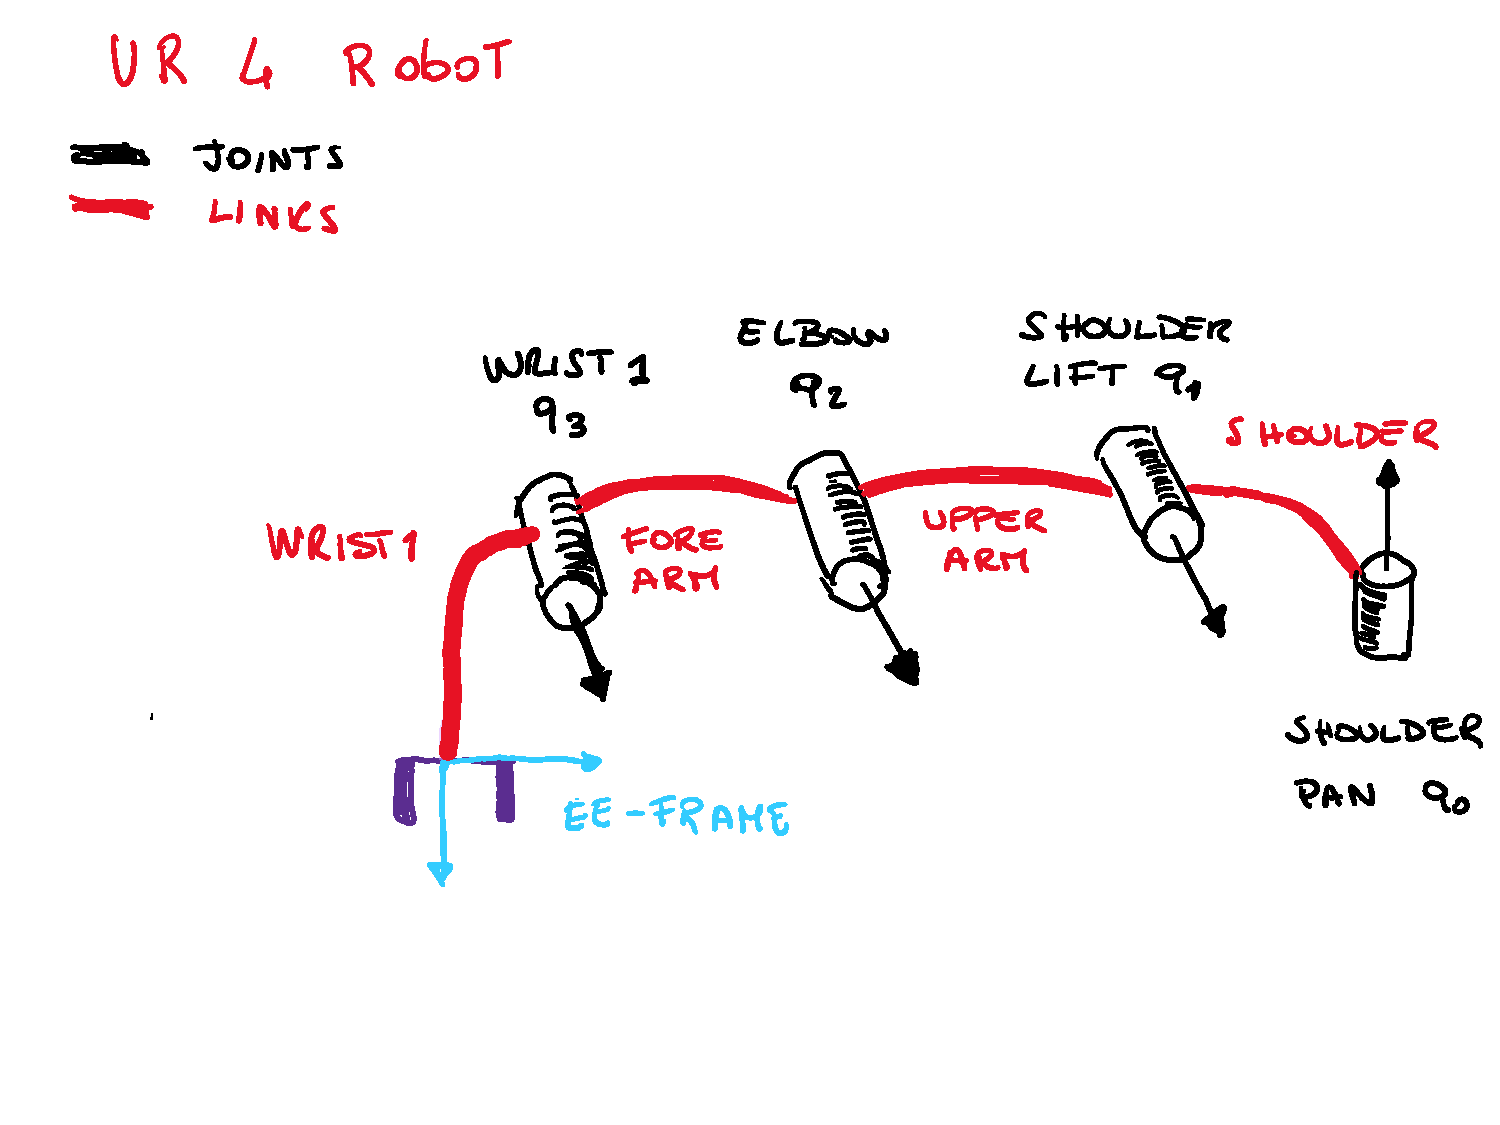
\includegraphics[width=10cm]{pics/ur4_Robot.pdf}
	\caption{Sketch of the UR4 robot kinematics}
	\label{fig:ur4_robot_kinematics}
\end{figure} 


\textbf{2.1 Direct kinematics (lecture E1).} The first step is to obtain the homogeneous transformation matrix from the world frame to the end-effector \prepos{T}{W}{e}. To do so, you will need to obtain the homogeneous transformation matrices from one link to the other (i.e., the local transformations \prepos{T}{W}{1}, \prepos{T}{1}{2}, \prepos{T}{2}{3}, \prepos{T}{3}{4} and \prepos{T}{4}{e}) and perform the composition of matrices. Modify the function \codeword{directKinematics} inside \codeword{kin_dyn_utils.py} to perform this computation. Hint: you can use the previously shown visualization tool to understand the  position and orientation of the different frames (remember to set joint positions to zero). 
You can alternative refer to Fig. \ref{fig:ur4_robot_kinematics} for a sketch of the kinematics and to Fig.  \ref{fig:ur4_tf} to check the locations of the  link frames.


\begin{figure}[bht]
	\centering
	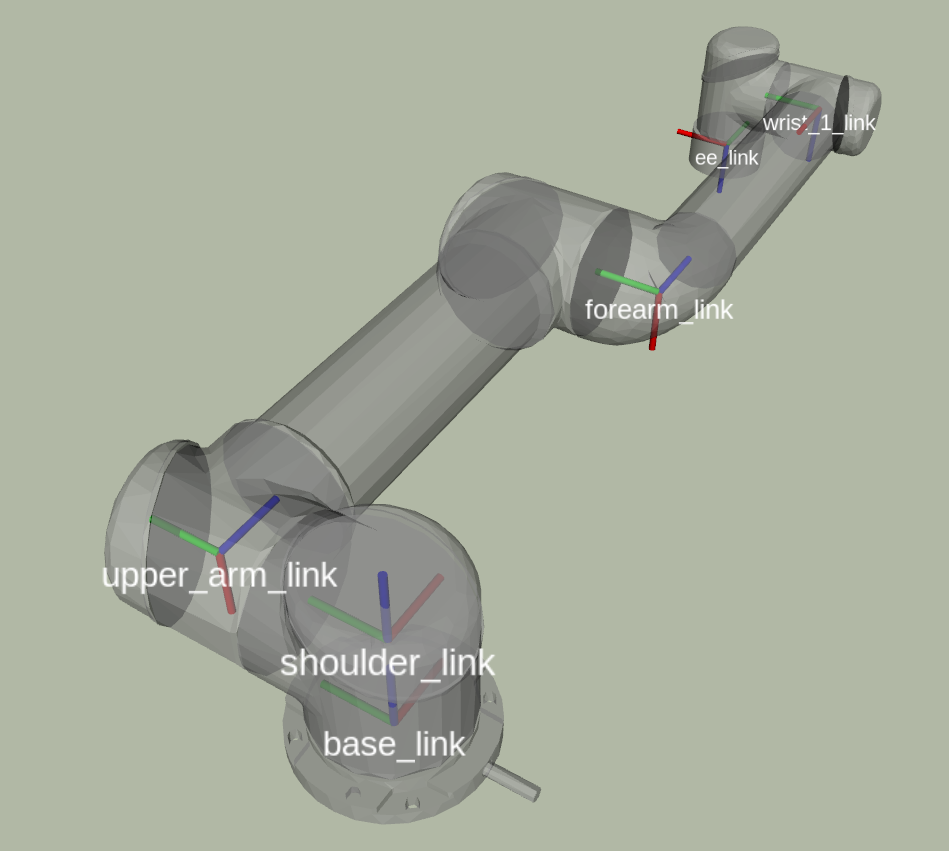
\includegraphics[width=10cm]{pics/ur4TF.png}
	\caption{UR4 Robot:  link frames locations}
	\label{fig:ur4_tf}
\end{figure} 


You can call the function inside the package kin\_dyn\_utils.py from the main in the \codeword{L1_1_kinematics.py} file. To verify the correctness of your direct kinematics function, compare the outputs with the ones from the built-in functions from Pinocchio for the position vector (\codeword{robot.framePlacement(q, frame_ee).translation}) and the rotation matrix (\codeword{robot.framePlacement(q, frame_ee).rotation}) (as seen in the file \codeword{L1_1_kinematics.py}) using different values for the positions of the joints (changing \codeword{q0} in \codeword{L1_conf.py}).\\





\textbf{2.2 Geometric Jacobian (lecture E3).} Now that you have devised a function to compute the direct kinematics, proceed to to compute the end-effector Jacobian of the manipulator by modifying the function \codeword{computeEndEffectorJacobian} in \codeword{kin_dyn_utils.py}. Recall that the expression to compute the geometric Jacobian is:
\begin{equation*}
	\mathbf{J} = \begin{bmatrix}
		\mathbf{J}_{P1} & \dots & \mathbf{J}_{Pi} \\
		\mathbf{J}_{O1} & \dots & \mathbf{J}_{Oi}
	\end{bmatrix}
\end{equation*}

where
\begin{equation*}
	\begin{bmatrix}
		\mathbf{J}_{Pi}\\
		\mathbf{J}_{Oi}
	\end{bmatrix} = 
	\begin{cases}
		\begin{bmatrix}
			\mathbf{z}_i \\
			\mathbf{0}
		\end{bmatrix} \text{   if $i$ is prismatic} \\
		\\
		\begin{bmatrix}
			\mathbf{z}_i \times (\preposm{p}{W}{e} - \preposm{p}{W}{i}) \\
			\mathbf{z}_i
		\end{bmatrix}\text{   if $i$ is revolute}
	\end{cases}
\end{equation*}

In our case all of the joints are revolute. Recall as well that in this expression vector $\mathbf{z}_i$ represents the moving axis of joint $i$ that drives link $i$, expressed in the world frame. As in the previous case, compare your results with the built-in function of Pinocchio:
\codeword{robot.frameJacobian(q, frame_ee, False, pin.ReferenceFrame.LOCAL_WORLD_ALIGNED) } for different values of \codeword{q}.\\

\textbf{2.3 Analytical Jacobian (lecture E3).} In the case we decide to parametrize our task variables representing the orientation with Euler Angles, we can obtain the Analytic Jacobian directly from the Geometric Jacobian via a simple transformation. Proceed to compute the analytical Jacobian $\mathbf{J}_a$ according to:
%
\begin{equation*}
	\mathbf{J}_a = \mathbf{T}_{RPY} \mathbf{J}
\end{equation*}
where $\mathbf{J}$ is the geometric Jacobian and $\mathbf{T}_a$ is the transformation matrix given by
\begin{equation*}
	\mathbf{T}_a = \begin{bmatrix}
		\mathbf{I} & \mathbf{0} \\
		\mathbf{0} & \mathbf{T}_{RPY}^{-1}
	\end{bmatrix}
\end{equation*}

where $\mathbf{T}_{RPY}^{-1}$ is the transformation matrix from angular velocity $\boldsymbol{\omega}$ to Euler angle rate $\dot{\mathbf{\Phi}}$, i.e.,
\begin{equation*}
	\boldsymbol{\omega} = \mathbf{T}_{RPY} \dot{\mathbf{\Phi}}
\end{equation*}

and implement it in the function \codeword{geometric2analyticJacobian}.\\




\textbf{2.4 Numerical inverse kinematics (lecture E4).} Now you have all the necessary ingredients to compute the manipulator's inverse kinematics. Since we have 4-DoF, the analytical solution of the inverse kinematics problems is not straightforward, so we suggest to take the iterative approach given by the algorithm described in Fig.~\ref{fig:CLIK}.  
%
\begin{figure}[bht]
	\centering
	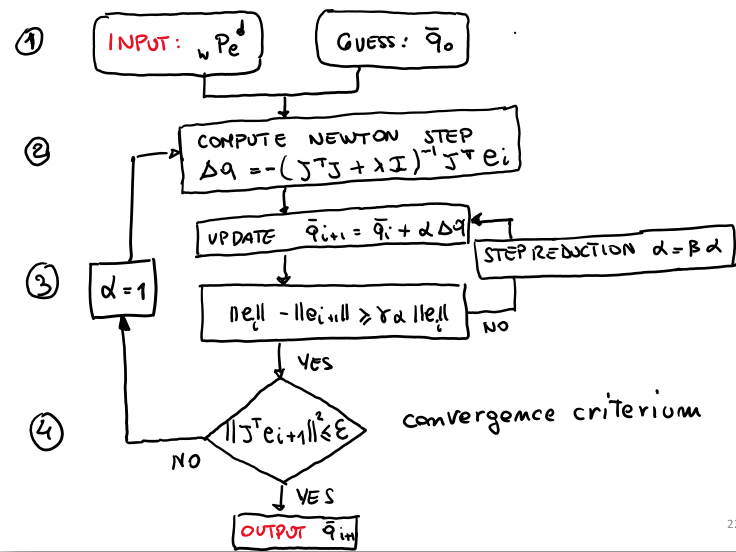
\includegraphics[width=8cm]{pics/flow_chart.png}
	\caption{Numerical inverse kinematics algorithm or closed-loop inverse kinematics (CLIK)}
	\label{fig:CLIK}
\end{figure}
%
To start simple, consider your task space variables to be the Cartesian space position (i.e., $x,y,z$) and the roll angle $\psi$ of the end-effector. 
Why can't the full orientation be defined in the task? (hint: check which row in the Jacobians goes to zero).
%You will need to adequately choose the rows of interest of the analytical Jacobian $\mathbf{J}_r$. 
Since we have 4 task variables and 4 DoFs then   $\mathbf{J}_a$ is a square matrix and we expect $\mathbf{J}_a^T\mathbf{J}_a$ to be always invertible (out of singularities).  After implementing your function, try to find the corresponding joint angles for $p = \mat{-0.5 & -0.2 & 0.5 & \frac{\pi}{3}}^T$, where the first three components are the $x$, $y$, $z$ Cartesian coordinates of the end-effector and the fourth component corresponds to the roll angle $\psi$ of the end-effector frame. Set your hyper-parameters for the algorithm as follows: $\alpha = 1$, $\epsilon = 1 \times 10^{-6}$ and $\beta = 0.5$ where $\beta$ is the coefficient of step-size reduction in the line search, and $\epsilon$ is the termination tolerance. 
First, implement the algorithm without line search (i.e., with constant step size $\alpha$) and then compare it with the adjustable step size. Is there any difference in the number of iterations?  (you should notice that the line search might take a smaller number of iterations, 10 instead of 35). What is the influence of the initial condition? 
Check that the algorithm converges to different joint configurations depending on how you initialize it and that the number of iterations changes. 
Try to set it in order to converge to the elbow up or elbow down configuration.  
%Are the output values for the trajectory "safe"? 

Using the joint angles coming out of the numerical inverse kinematics, compute the direct kinematics and obtain the error between the asked task space position and the computed one using the joint angles obtained from the inverse kinematics and verify the error is close to zero.  
%Then you  can compute the norm of the error between the position that was asked and the final position reached.
 

Despite the correct result (no error at the end-effector), 
you might notice that the values of the joint variables $q$ are very large. Why is this? 
You will have to implement a "wrapping" function to keep the joint angles between $-2\pi$ and $2\pi$. 

 
Now,  compare different outputs of the numerical inverse kinematics function  using the line search algorithm but limiting the maximum number of iteration to 3, 4 and 5, how much is the difference between the final position and the target? 

% Why is one closer than the other? (in this case the line search is closer to the final point). Try now increasing the maximum number of iterations to 15000 to see that the larger the number of iterations, the closer you get to $p$. 

Figure~\ref{fig:ik} shows the position of the robot after 3, 4 and 5 iterations.  
\begin{figure}[H]
	\centering
	\begin{subfigure}[b]{0.3\textwidth}
		\centering
		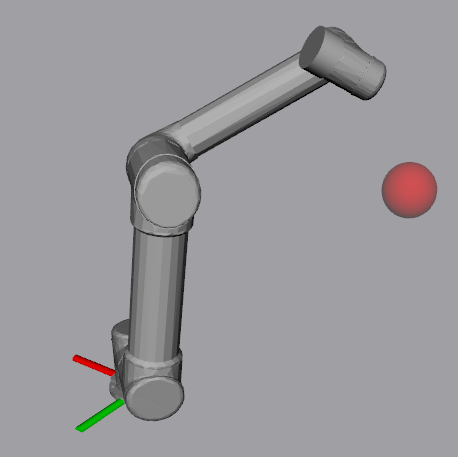
\includegraphics[height=\textwidth]{pics/3iters.png}
		\caption{Position after 3 iterations}
		\label{fig:3it}
	\end{subfigure}
	\begin{subfigure}[b]{0.3\textwidth}
		\centering
		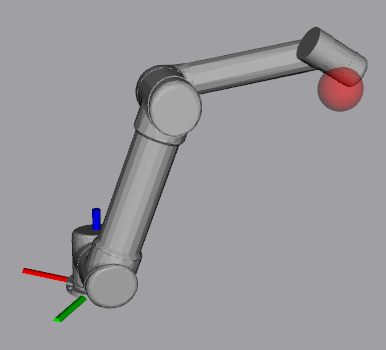
\includegraphics[width=\textwidth]{pics/4iters.png}
		\caption{Position after 4 iterations}
		\label{fig:4it}
	\end{subfigure}
	\begin{subfigure}[b]{0.3\textwidth}
		\centering
		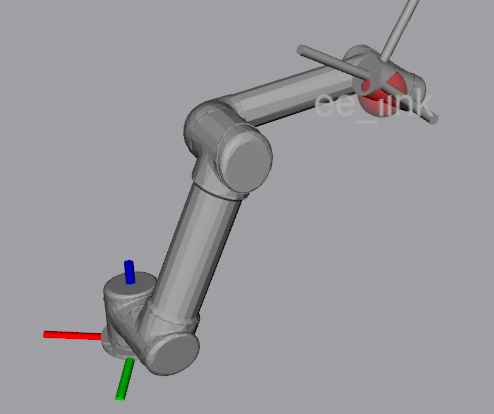
\includegraphics[height=\textwidth]{pics/5iters.png}
		\caption{Position after 5 iterations}
		\label{fig:5it}			
	\end{subfigure}
	\caption{Positions of the robot manipulator after 3,4, and 5 iterations of the numerical inverse kinematics}
	\label{fig:ik}
\end{figure} 
 
You can notice that the algorithm is converging very fast (the rate of convergence of Gauss-Newton method approaches the quadratic) and the robot is very close to  the target already after 4 iterations. 
 
Now, try to ask to reach a position of the end-effector \textit{outside} of the workspace, for example, $p = \mat{	-1.0 & -0.2 & 0.5 & \frac{\pi}{3}}^T$. Start without the line search, is the error going to zero? verify that the algorithm never converges (the maximum number of iterations is reached). If you enable the line search the robot tries to do "the best that he can" to reach the target, reducing the error, but still the maximum number of iteration is reached. Increasing the regularization term $\lambda$ (e.g. to 0.01) you can see that the gradient goes under the tolerance $\epsilon$ before reaching the maximum value of iterations (and the error will be minimum).





A limitation of this approach is that joint limits can be considered only at the end. An improvement would be to set up a \textit{constrained} optimization problem where we enforce the end-stop limits during the optimization.\\




\textbf{2.5 Fifth order joint polynomial trajectory.} Now that we have a function that computes the inverse kinematics, we can use our initial joint position $\mathbf{q}_0$(defined in the file \codeword{L1_conf.py}) and the final joint position vector $\mathbf{q}_f$ (computed with our numerical inverse kinematics function) to compute a trajectory and move from one point to the other. An easy way to do so is by using a fifth order \textit{polynomials} parameterized by time to represent the position and its derivatives (i.e., velocity and acceleration) of a given joint with respect to time, i.e.:
%
\begin{align*}
	q_i(t) &= a_0  + a_1 t +  a_2 t^2 + a_3 t^3 + a_4 t^4 + a_5 t^5\\
	\dot{q}_i(t) &= a_1 + 2 a_2 t + 3a_3 t^2 + 4 a_4 t^3 + 5 a_5 t^4\\
	\ddot{q}_i(t) &= 2 a_2 + 6 a_3 t + 12 a_4 t^2 + 20 a_5 t^3
\end{align*} 
%
we can then define a set of \textit{initial} and \textit{final} conditions for the joint variables $q_i$, $\dot{q}_i(t)$ and $\ddot{q}_i(t)$  to define the behavior of the trajectory. 
Using this \textit{boundary conditions} we can obtain the values of the coefficients $a_i$ by solving a $6\times 6$ linear system of equations (we have 6 equations and six unknowns). 
For the initial conditions we use the $\mathbf{q}_0$ and assume that the arm starts from a no-motion condition (i.e., $\dot{\mathbf{q}}_0 = \mathbf{0}$ and $\ddot{\mathbf{q}}_0 = \mathbf{0}$). 
For the final conditions we can use the joint values obtained by the inverse kinematics $\mathbf{q}_f$ and again assume that the robot will come to a full stop at the end of the motion (i.e., $\dot{\mathbf{q}}_f = \mathbf{0}$ and $\ddot{\mathbf{q}}_f = \mathbf{0}$). We initialize time $t_0 = 0$ and the final time $t_f$ we are free to choose (the shorter the time, the faster the robot will move). Let's select $t_f = 3s$. With these considerations, replacing $t = 0$ and $t = t_f$ the equations for initial and final conditions become (per joint):
%
\begin{align*}
	q_0 &= a_0  \\
	0 &= a_1 \\
	0 &= 2 a_2 \\
	q_f &= a_0  + a_1 t_f +  a_2 t_f^2 + a_3 t_f^3 + a_4 t_f^4 + a_5 t_f^5\\
	0 &= a_1 + 2 a_2 t_f + 3a_3 t_f^2 + 4 a_4 t_f^3 + 5 a_5 t_f^4\\
	0 &= 2 a_2 + 6 a_3 t_f + 12 a_4 t_f^2 + 20 a_5 t_f^3
\end{align*}
%
which can be rewritten in matrix form as: 
\begin{equation*}
	\begin{bmatrix}
		q_0 \\
		0 \\
		0 \\
		q_f \\
		0 \\
		0
	\end{bmatrix} =
	\begin{bmatrix}
		1 & 0   & 0     &       0 &        0 &     0 \\
		0 &   1 &     0 &       0 &        0 &     0 \\
		0 &   0 &     2 &       0 &        0 &     0 \\
		1 & t_f & t_f^2 &   t_f^3 &    t_f^4 & t_f^5 \\
		0 &   1 & 2 t_f & 3 t_f^2 &  4 t_f^3 & 5 t_f^4 \\
		0 &   0 &     2 &   6 t_f & 12 t_f^2 & 20 t_f^3
	\end{bmatrix}
	\begin{bmatrix}
		a_0 \\
		a_1 \\ 
		a_2 \\
		a_3 \\
		a_4 \\
		a_5
	\end{bmatrix}
\end{equation*}
Then we can pre-multiply both sides of the equation by the inverse of the square (6X6) matrix and on the right-hand side of the equation obtain the values for the coefficients of the polynomials.
With these coefficients we can generate the whole trajectory $q(t)$ starting for a time $t=0$ (where $q = q_0$) up to $t=t_f$ (where  $q = q_f$).

Implement this trajectory by modifying the function \codeword{fifthOrderPolynomialTrajectory}. Plot the trajectories by un-commenting the final lines of the file \codeword{L1_1_kinematics.py} and see if you notice any problem. Hint: you can set a \codeword{SLOW_FACTOR} of 50 to better see the motion. You will see that the robot is doing very strange loops. If you remove the \textit{wrapping} feature you will get something even worse. This is because of the initialization that has a strong influence. Try to initialize the ik with $q_0$ instead  than with $q_i$ and you will see that the trajectory improves significantly. However, if you set a target that is more far away (e.g.  $p^d_e =\mat{0.5 & -0.2 & 0.5}^T$) you will still see loops. 
Using this approach to generate the trajectory is simple, but has no guarantee on what is happening (e.g. where the end-effector will be) in between the initial and the final configurations.
Namely, you only now for sure where the end-effector is at the beginning and the end of the motion, which in real-life scenarios can lead to potential collisions or unwanted paths.



\textbf{Cartesian trajectory:} The solution is  to  design a trajectory directly in Cartesian space via parametric curves. For instance you can design a trajectory of a line in 3D Cartesian space parameterized by time and, for each position given by the curve along the trajectory, you will need to compute the inverse kinematics to provide the joint values (hint: you need to do it also at the velocity and at the acceleration level). As initial guess at each time instant you can set the configuration at the previous sample. Compare the results of the trajectory with respect to the one designed in 2.5.\\

\textbf{2.6 Dealing with the redundancy: the postural task.} 

Now, let's consider a ur5 robot with 6 DoFs. In this case we want to set \textit{only} the \textit{position} of the end-effector to be at $p^d_e =\mat{0.5 & -0.2 & 0.5}^T$. Hence, the robot (6 DoFs) becomes redundant for the task (3 variables) and we expect to have an  infinite number of solutions for the inverse kinematics problem. In particular the matrix $J^TJ$ becomes singular (semi-positive definite). Instead of using a regularization that would select a configuration that depends on the initial guess, we want to have a solution that is as  \textit{close} as possible to a desired configuration $q^p$ that we call \textit{postural} configuration. This could be, for instance, a configuration that tries to keep the joints in the middle of their range or minimize gravity torques. To achieve this,  we can implement a ``postural task'' at the kinematic level to solve the redundancy.
This will  select, among the infinite solutions, the one (joint configuration $\tilde{q}^\star$) that is closer (in an Euclidean sense) to the desired configuration $q^p$. 
To implement this, we setup the following optimization problem:

\begin{align*}
\tilde{q}^\star = \argmin_q \frac{1}{2} \left|\left| \mat{p(q) \\ w q } - \mat{p^d \\ w q^p }   \right|\right|^2 = \frac{1}{2} \left|\left| \mat{ e_x \\ e_q }   \right|\right|^2
\end{align*}

where $w$ is a scalar weight and $q^p$ the postural configuration. The solution of this optimization problem (which is still non convex do to the non linear dependency of $p_e$ from $q$) can be obtained through the Newton method, in a similar fashion to what we did in lab L1 - 2.4. The difference is the definition of the error $\bar{e} = \mat{e_x^T & e_q^T}^T$ (than now will be a $3+n$ vector) and the way the newton step $\Delta q$ is computed:


\begin{align*}
\Delta q &= -\left( \mat { J^T &  wI_{3 \times 3} } \underbrace{ \mat{J  \\ wI_{3 \times 3}}}_{\bar{J}} \right)^{-1} \left(J^T e_x + w^2e_q \right) \\
&= -\left( J^TJ + w^2I_{3 \times 3}\right)^{-1} \underbrace{ \left(J^T e_x + w^2 e_q \right) }_{\bar{J}^T\bar{e}}
\end{align*}

%old: note that we have a minus sign just because we defined differently $e_p$ (in Exe2.4 we were using $e_p = p^d- p$ instead of $e_p = p - p^d$).

So, with respect to the exercise 2.4: 1) we use $w^2$ instead of $\lambda $ to regularize the Hessian $\bar{J}^T\bar{J}$ and make it full rank and therefore invertible, 2) we added ad term $w^2 e_q $ in the computation of the Newton step, 3) we changed the stopping criteria of the IK algorithm checking if the norm of this new gradient $\bar{J}^T\bar{e}$ goes below $\epsilon$.
Set different postural configurations and observe that the optimal configuration is the one that places the end-effector in the desired position and is close to the postural  configuration selected.
\\

\section{Robot dynamics}

In this last part of the assignment we will use the Recursive Newton-Euler Algorithm (RNEA) to compute the robot dynamics without any joint torque. We will then proceed to compute each of the terms in the dynamics equation as shown during lecture F1.2.  We will start by writing our own function for the forward and backward passes of the RNEA and compute each of the terms of the dynamics equation. Then we will use the previously computed terms to obtain the forward dynamics (i.e., joint accelerations) and integrate them once to obtain velocity and twice  for position, using a forward/explicit Euler scheme. We will then compare our results with the built in functions of Pinocchio.





For this part of the assignment, we will use these three main files: 
\begin{itemize}
	\item \codeword{LOCOSIM/robot_control/L1_2_dynamics.py} (Main file to run the visualization and the exercises)
	\item \codeword{LOCOSIM/robot_control/L1_conf.py} (Initializations of variables and simulaion parameters)
	\item \codeword{LOCOSIM/robot_control/base_controller/utils/kin_dyn_utils.py} (Kinematics and dynamics functions)
\end{itemize}


\textbf{3.1 Build the function for the RNEA (lecture F1.2).} Write a function that computes the forward and backward passes of the RNEA in the case of revolute joints, \codeword{RNEA}. We will use the following equations from lecture F1.2. Refer to Figure \ref{fig:rnea} for variable definitions.


\begin{figure}[H]
	\centering
	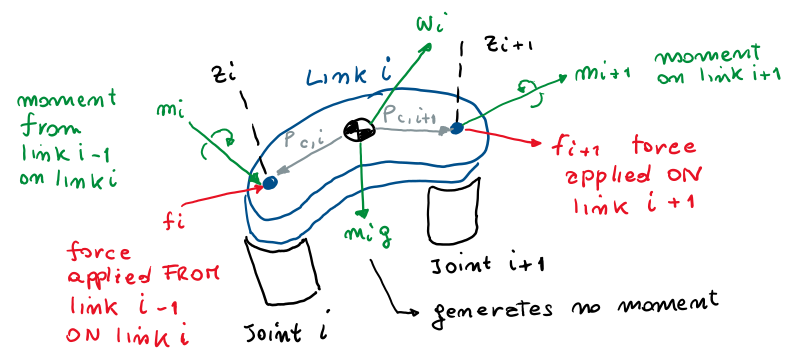
\includegraphics[width=12cm]{pics/rnea.png}
	\caption{Sketch of a link $i$ supported by joint $i$.}
	\label{fig:rnea}
\end{figure}

 So, for the forward pass we have\footnote{all quantities in both the forward and backward passes are expressed with respect to the world frame}:
\begin{align*}
	\boldsymbol{\omega}_i &= \boldsymbol{\omega}_{i-1} + \dot{\mathbf{q}}_i \mathbf{z}_i \\
%	
	\dot{\boldsymbol{\omega}}_i &= \dot{\boldsymbol{\omega}_{i-1}} + \ddot{\mathbf{q}}_i \mathbf{z}_i + \dot{\mathbf{q}}_i \boldsymbol{\omega}_{i-1} \times \mathbf{z}_i \\
%	
	\mathbf{v}_i &= \mathbf{v}_{i-1} + \boldsymbol{\omega}_{i-1} \times \mathbf{p}_{i-1,i} \\
%	
	\mathbf{a}_i &= \mathbf{a}_{i-1} + \dot{\boldsymbol{\omega}}_{i-1} \times \mathbf{p}_{i-1,i} + \boldsymbol{\omega}_{i-1} 	\times (\boldsymbol{\omega}_{i-1} \times \mathbf{p}_{i-1,i}) \\
%	
	\mathbf{a}_{ci} &= \mathbf{a}_{i} + \dot{\boldsymbol{\omega}}_{i} \times \mathbf{p}_{i,c} + \boldsymbol{\omega}_{i} 	\times (\boldsymbol{\omega}_{i} \times \mathbf{p}_{i,c})
\end{align*} 
where the last equations is the acceleration of the CoM, and vector $\mathbf{p}_{i,c}$ is the vector from joint frame $i$ to the CoM frame. This expression will be used to compute the forces and moments along the entire chain. It is important to note that the forward pass will be computed from the base link, which is not moving and it is only subject to the acceleration of gravity (i.e., $\boldsymbol{\omega}_0 = 0$, $\dot{\boldsymbol{\omega}}_0 = 0$, $\mathbf{v}_0 = 0$ and $\mathbf{a}_0 = -\mathbf{g}$). This simplifies the computation of the forces since the acceleration of gravity is already considered in the forward pass. For the backward pass, we will begin our computation from the end-effector frame. Consider that if the end effector is performing free-motion, then the forces and moments are equal to zero (i.e., $\mathbf{f}_{ee} =0$ and $\mathbf{m}_{ee} = 0$), however, if the end-effector is in contact with an object, a measurement or approximation of the forces and moments is needed. The backward pass equations for the moments and forces are
\begin{align*}
	\mathbf{f}_i &= \mathbf{f}_{i+1} + \mathbf{m}_i\mathbf{a}_{ci} \\
	\mathbf{m}_i &= \mathbf{m}_{i+1} - \mathbf{p}_{c,i} \times \mathbf{f}_i + \mathbf{p}_{c,i+1} \times \mathbf{f}_{i+1} + \mathbf{I}_i \dot{\boldsymbol{\omega}}_i + \boldsymbol{\omega}_i  \times \mathbf{I}_i \boldsymbol{\omega}_i
\end{align*}
Remember that all quantities are expressed with respect to the world, so you will need to provide appropriate transformations for the parameter vectors and matrices (e.g., the position of the CoM $\mathbf{p}_{ci}$ and the inertia tensor $\mathbf{I}_i$). The function \codeword{RNEA} should receive as input arguments the gravity vector $\mathbf{g}_0$ ($\begin{bmatrix}
	0 & 0 & -9.81
\end{bmatrix}^{\top}$), the vector of current joint positions $\mathbf{q}$, the vector of current joint velocities $\dot{\mathbf{q}}$ and the vector of current joint accelerations $\ddot{\mathbf{q}}$, i.e.,
\codeword{RNEA(g0,q,qd,qdd)}. \\

\textbf{3.2 Compute each of the terms of the dynamics equation (lecture F1.2). } Create functions to compute the vector of gravitational force $\mathbf{g}$, the joint space inertia matrix $\mathbf{M}$, and the vector of Coriolis and centrifugal terms $\mathbf{c}$. Remember that the RNEA function previously written can be used to obtain all of these terms by setting some quantities to 0. In essence, compute the gravity vector through the previous function by setting its arguments as \codeword{RNEA(g0,q,0,0)}, the vector of Coriolis and centrifugal forces with \codeword{RNEA(0,q,qd,0)} and each of the columns of the joint space inertia matrix with \codeword{RNEA(0,q,0,ei)}, where \codeword{ei} is a vector to select the i-th column of $\mathbf{M}$.\\


\textbf{3.3 Compute the robot joint accelerations (lecture F1.2).} Now that the equations of motion can be computed, simulate the robot dynamics under zero joint torque. To do this, you need to obtain the joint acceleration based on the equations of motion, namely:
%
\begin{equation*}
	\ddot{\mathbf{q}} = \mathbf{M}^{-1} (\boldsymbol{\tau} - \mathbf{g} - \mathbf{c})
\end{equation*}

with $\boldsymbol{\tau} = 0$ (for the time being). \\




\textbf{3.4 Simulate the robot dynamics using a forward Euler scheme (lecture F1.2).} 
With the previously computed joint acceleration, we can integrate once to obtain joint velocity and twice for position. 
Implement an improved forward/explicit Euler integration scheme in the included \codeword{while} loop in the provided main file to run your visualization \codeword{LOCOSIM/robot_control/L1_2_dynamics.py} by using the following equations:
\begin{align*}
	\dot{\mathbf{q}}(t  + \delta t) &= \dot{\mathbf{q}} (t) + \ddot{\mathbf{q}}(t) \delta t \\
	\mathbf{q}(t +\delta t) &= \mathbf{q}(t) + \dot{\mathbf{q}} (t) \delta t + \frac{\delta t^2}{2}\ddot{\mathbf{q}}(t)
\end{align*}
 where $\delta t$ is the time step of our simulation. Check the visualizer, you will see the robot falling 
 but never stopping, why is this the case? Is this realistic? What can be done to stop the motion after a while?. \\ 
 
\textbf{3.5 Add a damping term to the equation.} 
The robot is not stopping since there is no friction or damping that allows the joint velocities to come to a stop. 
Implement a damping term by defining $\mathbf{\tau}$ as
\begin{equation*}
	\boldsymbol{\tau} = -b\dot{\mathbf{q}}
\end{equation*} 
where $b$ is the damping coefficient of the joints. For now we keep $b$ as a scalar, however, you can set different damping coefficients for each of the joints. Try different values of $b$ and visualize the behavior of the robot changing.\\


\textbf{3.6 Compare results against Pinocchio.} Compute the terms of the dynamics equation $\mathbf{M}$, $\mathbf{c}$ and $\mathbf{g}$ using the built in functions from Pinocchio. To compute $\mathbf{g}$ use the following function: \codeword{robot.gravity(q)}, which takes as only argument the vector of joint positions. To compute $\mathbf{M}$ use: \codeword{robot.mass(q, False)}\footnote{For the functions of the mass and nonlinear terms the second argument is a boolean related to the update of the joint variables, in our case we are keeping it as false since we are updating the joint states manually}. In the case of vector $\mathbf{C}$, Pinocchio only provides the sum $\mathbf{h} = \mathbf{c} +  \mathbf{g}$ through the function: \codeword{robot.nle(q, qd, False)}\footnote{Nle stands for non linear effects.}. Run again the simulation using Pinocchio and verify that the outputs of the function that you wrote coincides with those of the built-in functions. Now remove entirely the implementation with your functions and visualize the robot falling. You will notice that the robot is moving  faster that with your own implementation. Why is this the case?  This is mainly due to the fact that Pinocchio is implemented in C++ but used in Python through bindings and because our implementation is done with respect to the world frames. Whereas in Pinocchio computations are done  with respect to the link frame, and this results in "sparser" matrix multiplications (i.e. the inertia tensors are full of zeros and this results in faster matrix multiplications).



\end{document}





